\begin{frame}[t]{Model and Mechanism}
\small
\begin{columns}[T,onlytextwidth]
\begin{column}{0.55\textwidth}
\textbf{Environment}
\begin{itemize}
    \item Two Egyptian regions: QIZ-eligible regions $(Q)$ and non-QIZ regions $(N)$.
    \item Two sectors in the current quantitative version: textiles/apparel $(T)$ and other manufacturing $(O)$.
    \item Three destinations: Egypt, United States, and rest of world.
\end{itemize}

\textbf{Firm decisions}
\begin{itemize}
    \item Firms draw productivity and choose whether to serve each destination.
    \item QIZ-region firms can comply with rules of origin to access the US duty free.
    \item US access can trigger upgrading, which raises productivity in all destinations.
\end{itemize}

\textbf{General equilibrium}
\begin{itemize}
    \item Wages, entry, price indices, and labor reallocation are solved jointly.
    \item This lets the model map firm-level compliance to wages, exports, and welfare.
\end{itemize}
\end{column}
\begin{column}{0.43\textwidth}
\centering
\includegraphics[width=\linewidth]{qiz_model_diagram}
\vspace{0.4em}

\footnotesize
Key margin: compliance lowers the US tariff wedge but raises required Israeli-input use.
\end{column}
\end{columns}
\end{frame}

\begin{frame}[t]{QIZ vs No QIZ: Main Results}
\small
\begin{columns}[T,onlytextwidth]
\begin{column}{0.62\textwidth}
\centering
\renewcommand{\arraystretch}{1.12}
\begin{tabular}{lrrr}
\hline
\textbf{Outcome} & \textbf{No QIZ} & \textbf{QIZ} & \textbf{\% change} \\
\hline
Total exports to US & 46.35 & 45.11 & -2.7 \\
Total exports to non-US & 123.22 & 122.88 & -0.3 \\
QIZ-region exports to US & 34.00 & 27.11 & -20.3 \\
Non-QIZ-region exports to US & 12.34 & 18.00 & +45.8 \\
\hline
\end{tabular}
\end{column}
\begin{column}{0.34\textwidth}
\textbf{Complier moments}
\begin{itemize}
    \item Same-type compliers export \textbf{224.6\%} more to the US under QIZ.
    \item The same firms export \textbf{183.3\%} more to non-US markets.
    \item The model therefore fits the micro mechanism much better than the aggregate reallocation moments.
\end{itemize}
\end{column}
\end{columns}

\vspace{0.4em}
\begin{columns}[T,onlytextwidth]
\begin{column}{\textwidth}
\footnotesize
Takeaway: QIZ works primarily through a strong complier margin. In the richer economy-wide ROO version, the aggregate response mainly reflects reallocation across regions and sectors rather than a large aggregate export boom.
\end{column}
\end{columns}
\end{frame}

\begin{frame}[t]{Counterfactual: Relaxing the Input Requirement}
\small
\textbf{Policy experiment}
\begin{itemize}
    \item Vary the required Israeli input share $\gamma$ economy-wide.
    \item Re-solve the full equilibrium for each value of the common ROO requirement.
\end{itemize}

\textbf{What matters most}
\begin{itemize}
    \item Lower $\gamma$ raises compliance and reduces Israeli-input use per unit of exports.
    \item It also operates through two margins: stronger incumbent compliers and new compliers in lower-tariff sectors.
\end{itemize}

\vspace{0.4em}
\begin{columns}[T,onlytextwidth]
\begin{column}{0.48\textwidth}
\centering
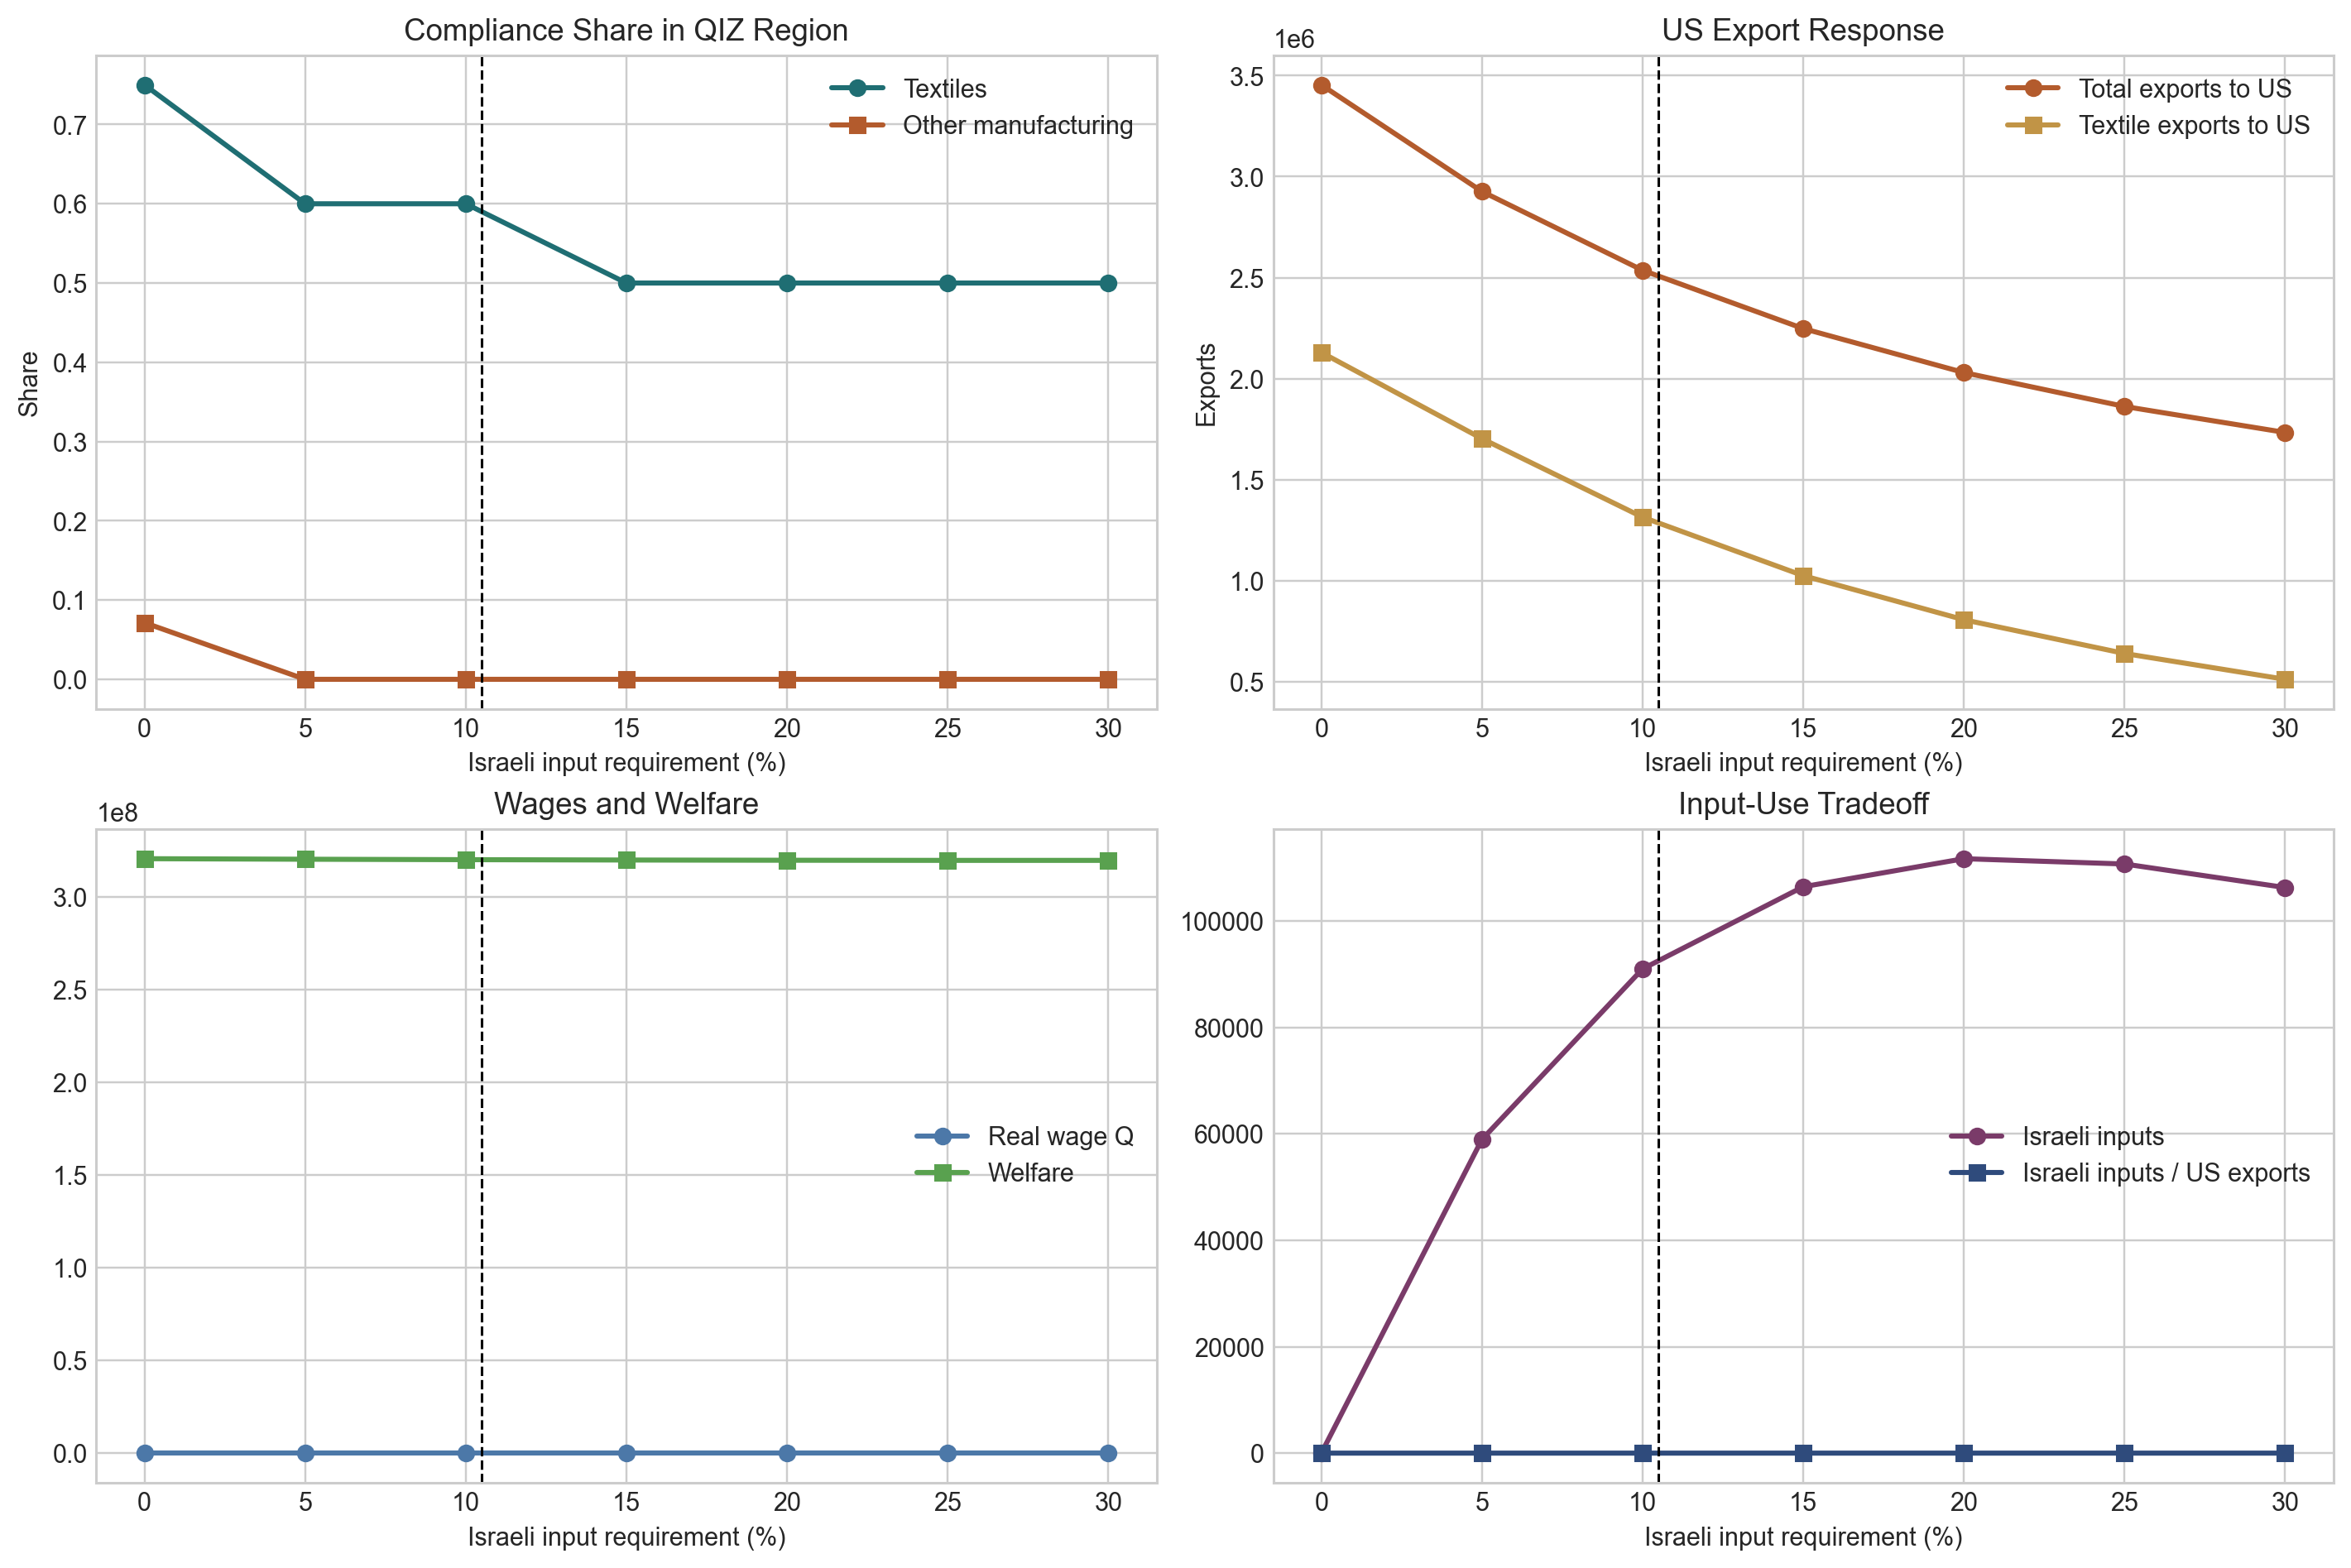
\includegraphics[width=\linewidth]{presentation_outputs/presentation_gamma_tradeoff}
\vspace{0.2em}

\footnotesize
Lower input requirements increase compliance and slightly improve wages and welfare.
\end{column}
\begin{column}{0.48\textwidth}
\centering
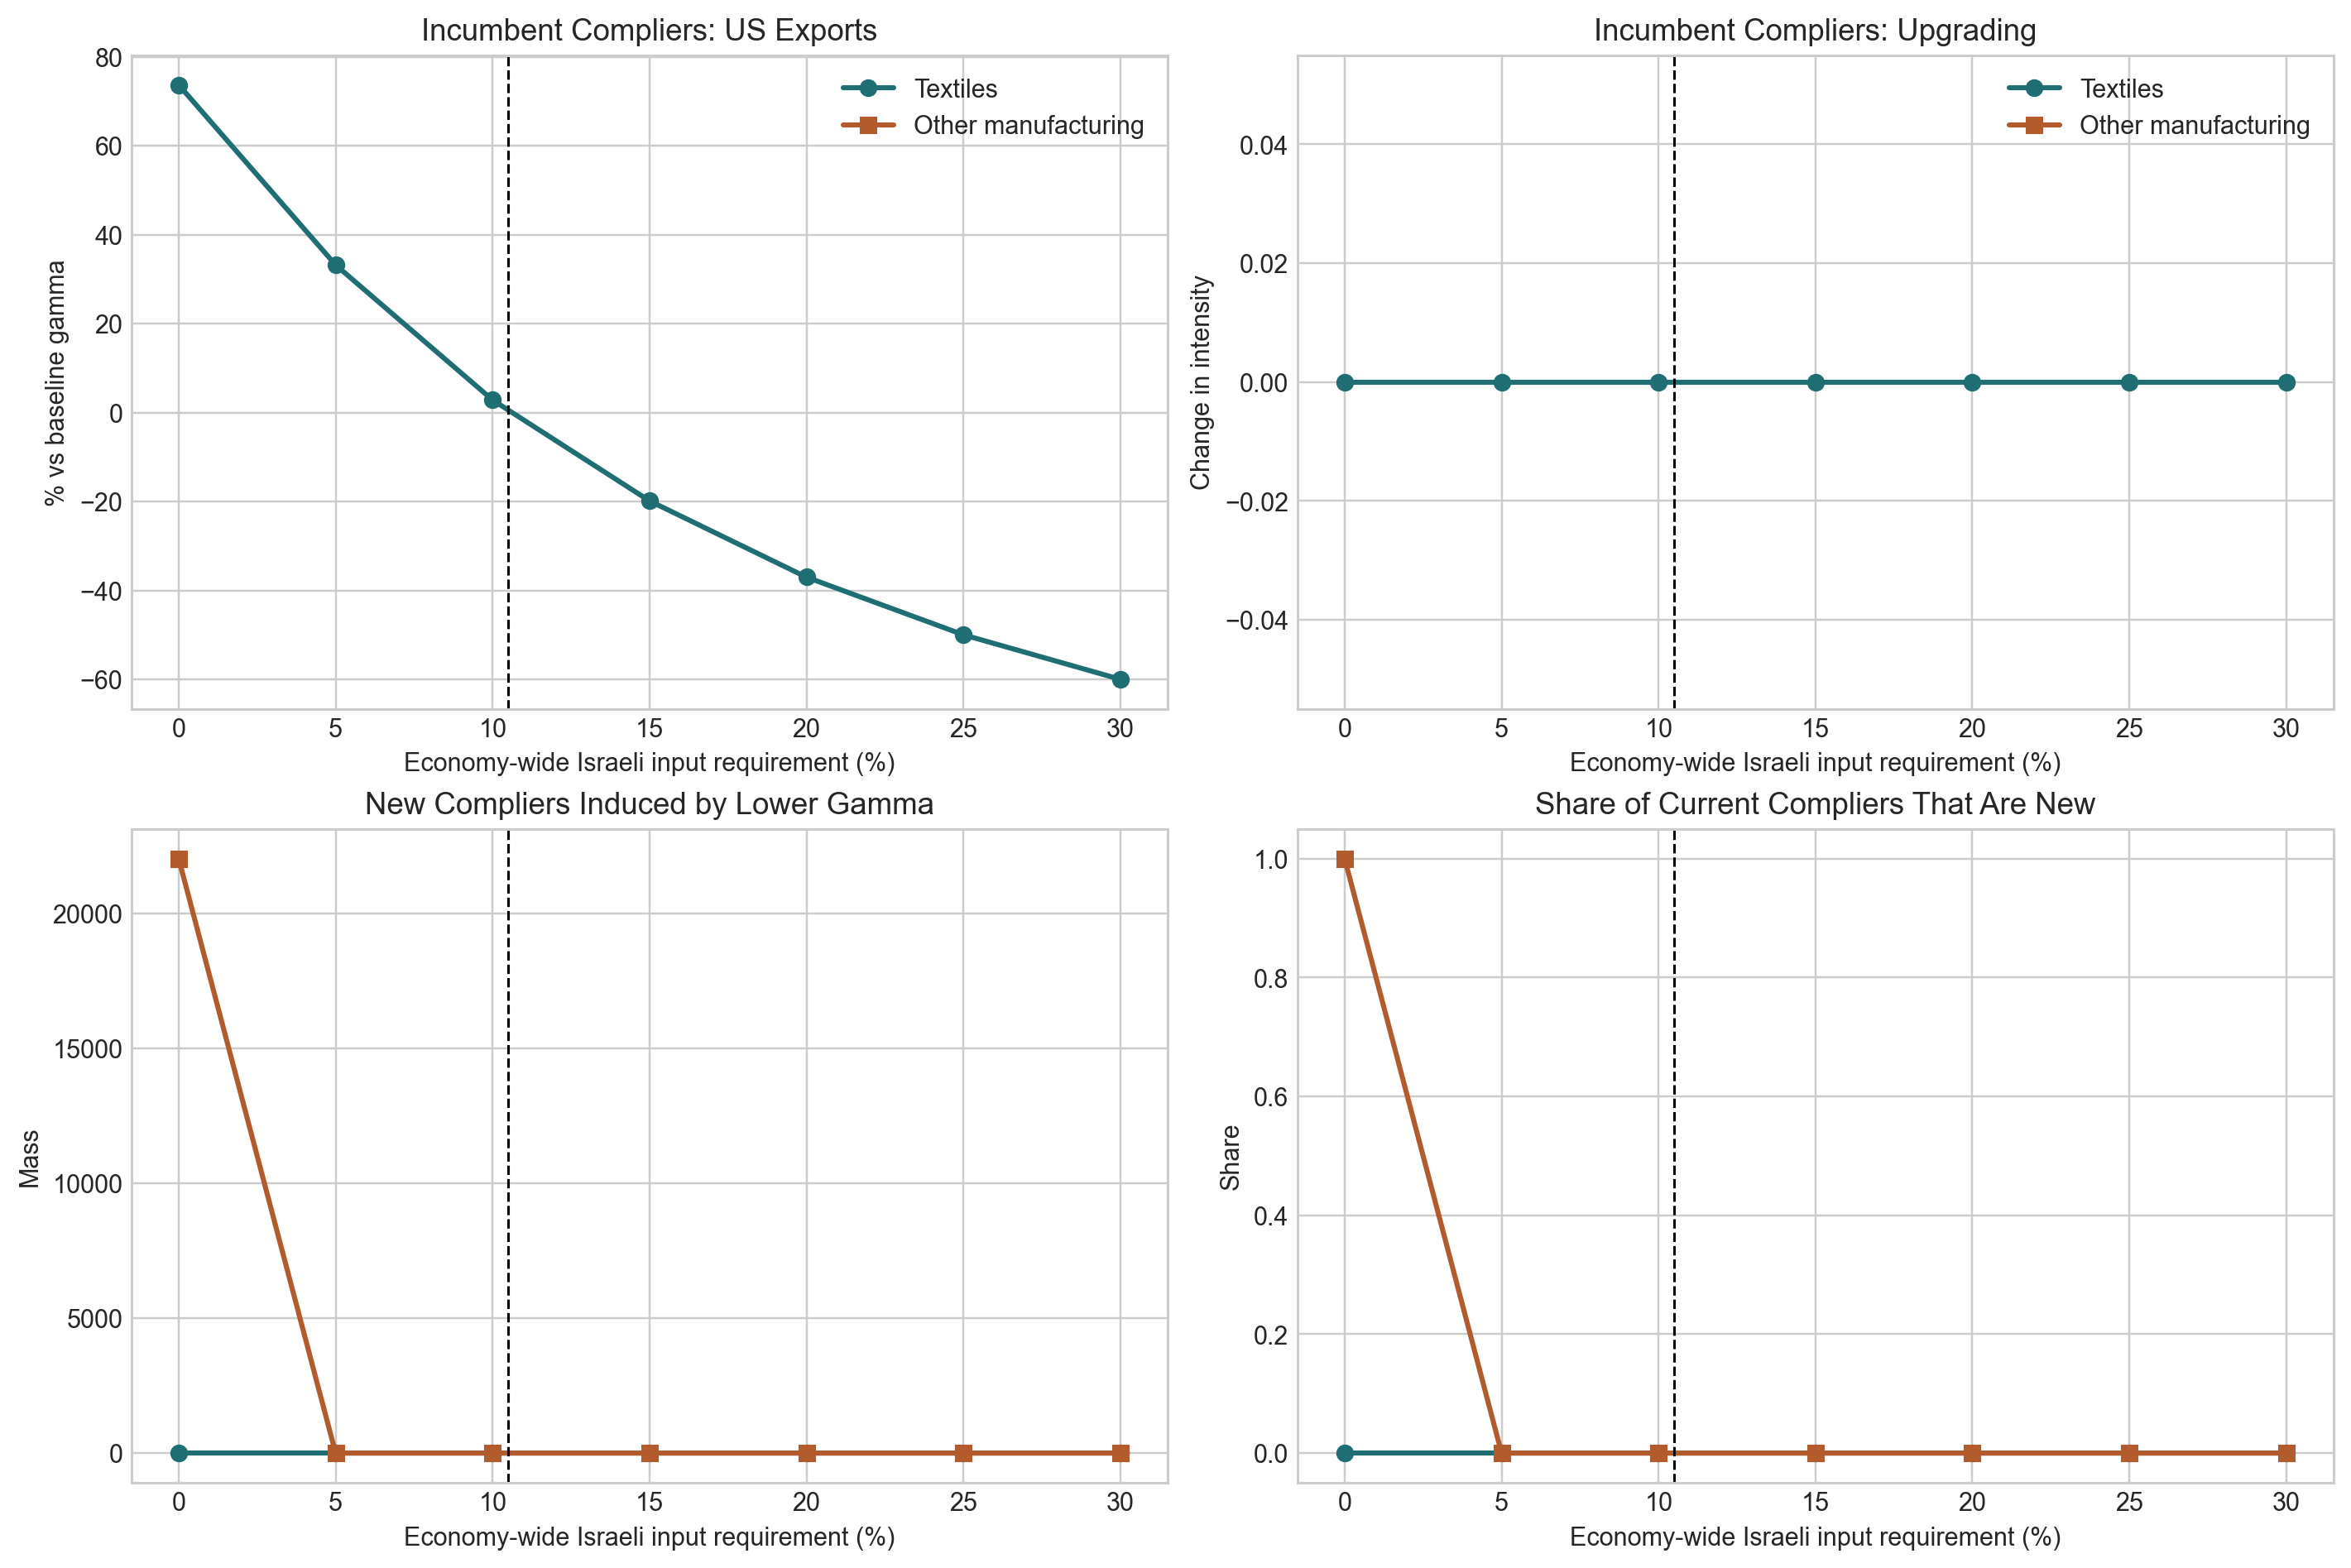
\includegraphics[width=\linewidth]{presentation_outputs/presentation_gamma_mechanism}
\vspace{0.2em}

\footnotesize
At low $\gamma$, new compliance appears in other manufacturing as well as textiles.
\end{column}
\end{columns}
\end{frame}
